\documentclass[12pt,a4paper,oneside,openany,oneauthor,masterthesis,deansoffice]{mfipl}

\usepackage{float}
\usepackage{graphicx}
\usepackage{clrscode}
\usepackage{latexsym}
\usepackage{amsmath}
\usepackage{booktabs}


\begin{document}

\section*{Zadanie 1 -- Erozja obrazu binarnego}

\subsection*{(a) Erozja zadanym elementem strukturalnym}

\begin{figure}[H]
\centering
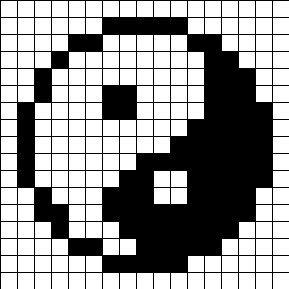
\includegraphics[width=0.32\textwidth]{zad1/yinyang.png}
\hfill
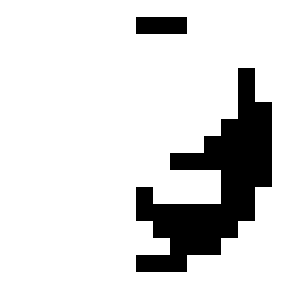
\includegraphics[width=0.32\textwidth]{zad1/erozja-wynik.png}
\hfill

\includegraphics[width=0.32\textwidth]{zad1/erozja-imagej.png}
\caption{Od lewej: obraz wejściowy \texttt{yinyang.png}, wynik własnej erozji (SE poziomy $1\times3$, anchor po prawej), wynik erozji w ImageJ.}
\end{figure}

\subsection*{(b) Porównanie z ImageJ}

ImageJ w operacji \texttt{Process $\to$ Binary $\to$ Erode} stosuje na sztywno kwadratowy element strukturalny $3\times3$ z punktem centralnym w środku. Z tego powodu:
\begin{itemize}
    \item własna erozja eliminuje tylko piksele, którym brakuje sąsiada po lewej (w kierunku zgodnym z orientacją SE) -- pozostają fragmenty pionowe;
    \item erozja ImageJ eliminuje piksele, którym brakuje jakiegokolwiek z ośmiu sąsiadów -- pozostaje znacznie mniejsza ,,rdzennie wewnętrzna'' część obiektu.
\end{itemize}
Różnica obrazów wyjściowych wynika więc z różnego kształtu i rozmiaru SE oraz z różnego położenia punktu centralnego.

\section*{Zadanie 2 -- Dylatacja obrazu binarnego}

\subsection*{(a) Dylatacja zadanym elementem strukturalnym}

\begin{figure}[H]
\centering
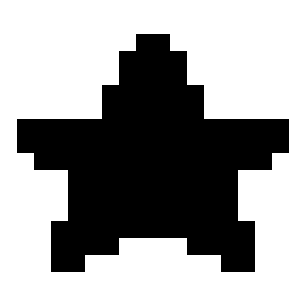
\includegraphics[width=0.32\textwidth]{zad2/dylatacja.png}
\hfill

\includegraphics[width=0.32\textwidth]{zad2/dylatacja-imagej.png}
\caption{Od lewej: obraz wejściowy, wynik dylatacji w ImageJ ($3\times3$). Wynik własnej dylatacji jest zapisany w pliku \texttt{dylatacja\_wynik.txt}.}
\end{figure}

\subsection*{(b) Porównanie z ImageJ}

ImageJ wykonuje dylatację z kwadratowym SE $3\times3$ z punktem centralnym w środku, co powiększa obraz symetrycznie we wszystkich kierunkach. Zastosowany w naszej implementacji SE $2\times2$ z anchorem $(0,0)$ powiększa obraz asymetrycznie -- jedynie w prawo i w dół. Wynikowy obraz jest więc przesunięty względem oryginału, a jego pogrubienie nie jest jednakowe wzdłuż każdej osi.

\section*{Zadanie 3 -- Identyfikacja operacji na obrazach $A \to B$}

\paragraph{(a) Operacja.}
Skoro pojedyncze piksele zostały rozmnożone w stały, identyczny wzór, jest to \textbf{dylatacja} obrazu $A$ elementem strukturalnym $S$ odpowiadającym wzorowi widocznemu w $B$.

\paragraph{(b) Element strukturalny.}
Wzór ma postać $5\times5$ z punktem centralnym wewnątrz figury:
\[
S = \begin{pmatrix}
0 & 0 & 0 & 0 & 1 \\
1 & 0 & 0 & 1 & 0 \\
1 & 0 & 1 & 0 & 0 \\
1 & 1 & 0 & 0 & 0 \\
1 & 1 & 1 & 1 & 1
\end{pmatrix}, \quad \text{anchor} = (2,2).
\]
Implementacja i sprawdzenie -- \texttt{zad3/dylatacja.py}. Wynik własny (\texttt{dylatacja\_wynik.txt}) jest identyczny z obrazem $B$.

\begin{figure}[H]
\centering
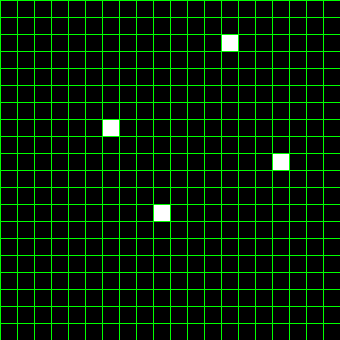
\includegraphics[width=0.40\textwidth]{zad3/Untitled-1.png}
\hfill
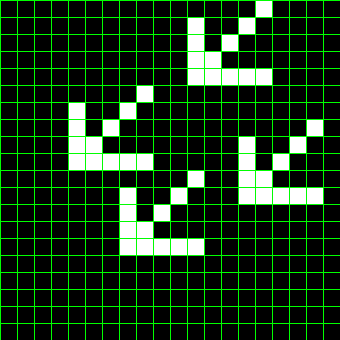
\includegraphics[width=0.40\textwidth]{zad3/dylatacja_wynik.png}
\caption{Po lewej: obraz wejściowy $A$. Po prawej: obraz $B$ -- wynik dylatacji obrazu $A$ podanym SE z centrum $(2,2)$.}
\end{figure}

\section*{Zadanie 4 -- Identyfikacja operacji na obrazach $A \to B$}

\paragraph{(a) Operacja.}
W $B$ nie pojawiają się piksele spoza $A$, a obiekty zostały zredukowane do pikseli, dla których określony układ sąsiadów był w $A$ równy $1$. Jest to zatem \textbf{erozja} obrazu $A$ elementem strukturalnym $S$.

\paragraph{(b) Element strukturalny.}
Aby pozostały tylko piksele o spełnionym warunku diagonalnym (piksel i jego prawy-dolny sąsiad oba równe $1$), zastosowano SE $2\times2$ z dwoma punktami na przekątnej i centrum w prawym-dolnym rogu:
\[
S = \begin{pmatrix} 1 & 0 \\ 0 & 1 \end{pmatrix}, \quad \text{anchor} = (1,1).
\]

\begin{figure}[H]
\centering

\includegraphics[width=0.40\textwidth]{zad4/Untitled-1.png}
\hfill
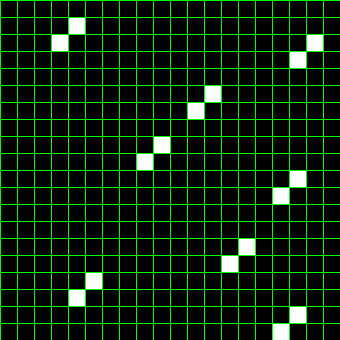
\includegraphics[width=0.40\textwidth]{zad4/erozja_wynik.png}
\caption{Po lewej: obraz wejściowy $A$. Po prawej: obraz $B$ -- wynik erozji obrazu $A$ ukośnym SE $\begin{pmatrix}1&0\\0&1\end{pmatrix}$ z centrum $(1,1)$.}
\end{figure}

\section*{Zadanie 5 -- Hit-or-Miss: lewe górne rogi obiektów}

Oznaczając \emph{don't care} jako $\times$, otrzymujemy:
\[
S = \begin{pmatrix}
0 & 0 & \times \\
0 & 1 & 1 \\
\times & 1 & \times
\end{pmatrix}, \quad \text{anchor} = (1,1).
\]

\begin{figure}[H]
\centering
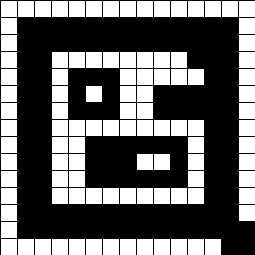
\includegraphics[width=0.40\textwidth]{zad5/smile.png}
\hfill
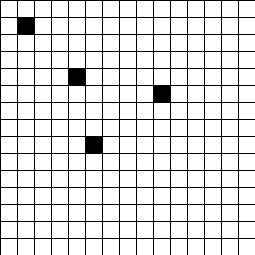
\includegraphics[width=0.40\textwidth]{zad5/hit_or_miss_wynik.png}
\caption{Po lewej: obraz wejściowy \texttt{smile.png}. Po prawej: wynik Hit-or-Miss -- pojedyncze piksele w lewych górnych rogach wszystkich obiektów.}
\end{figure}

\section*{Zadanie 6 -- Szkieletowanie}

\subsection*{(a) Szkieletowanie w ImageJ na obrazie \texttt{RoweremNaUG.png}}

\begin{figure}[H]
\centering
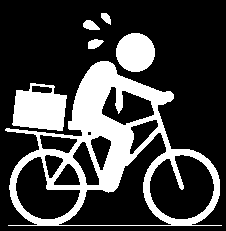
\includegraphics[width=0.45\textwidth]{zad6/RoweremNaUG.png}
\hfill
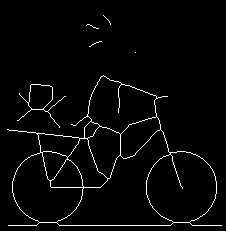
\includegraphics[width=0.45\textwidth]{zad6/RoweremNaUG-szkielet.png}
\caption{Obraz wejściowy oraz wynik operacji \texttt{Skeletonize} w ImageJ.}
\end{figure}

Algorytm dobrze radzi sobie z kształtami wydłużonymi i jednolitymi (rama roweru, sylwetka rowerzysty), natomiast problematyczne są kształty, których ,,oś środkowa'' nie jest jednoznacznie określona

\subsection*{(b) Zhang-Suen na wzorach $3\times3$ vs.\ szkieletowanie w ImageJ}

\begin{figure}[H]
\centering
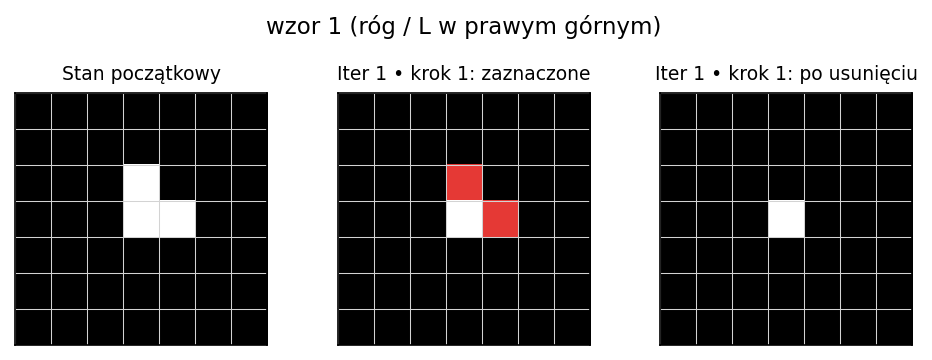
\includegraphics[width=0.9\textwidth]{zad6/a.png}
\caption{Wzór 1 -- róg / L w prawym górnym; krok 1 pierwszej iteracji usuwa dwa piksele, pozostaje pojedynczy punkt.}
\end{figure}

\begin{figure}[H]
\centering
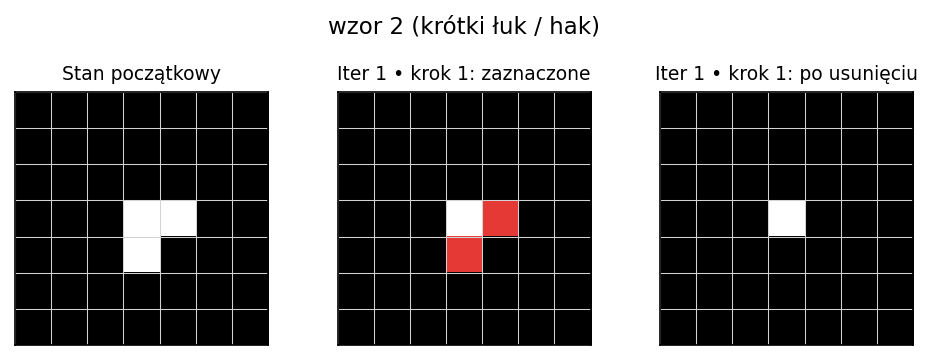
\includegraphics[width=0.9\textwidth]{zad6/b.png}
\caption{Wzór 2 -- krótki łuk; algorytm usuwa dwa piksele tworzące zakrzywienie, zostaje pojedynczy punkt.}
\end{figure}

\begin{figure}[H]
\centering
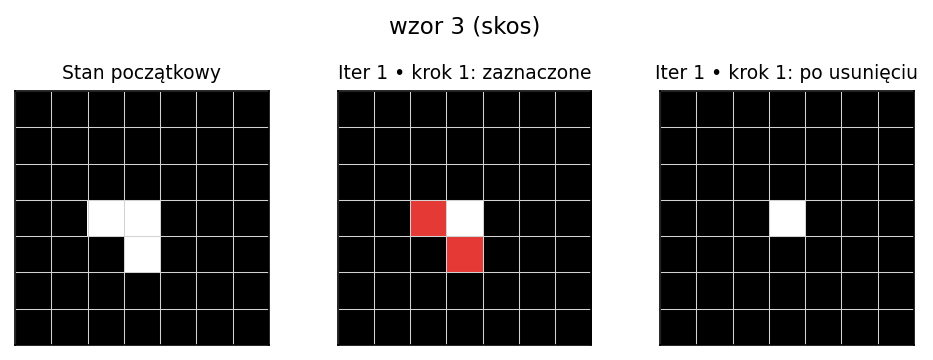
\includegraphics[width=0.9\textwidth]{zad6/c.png}
\caption{Wzór 3 -- skos; po pierwszym kroku zostaje pojedynczy piksel.}
\end{figure}

\begin{figure}[H]
\centering
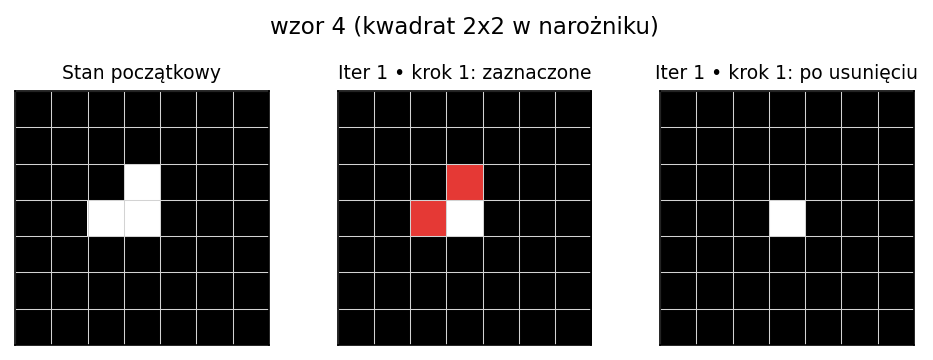
\includegraphics[width=0.9\textwidth]{zad6/d.png}
\caption{Wzór 4 -- kwadrat $2\times2$ w narożniku; po pierwszym kroku z czteropikselowego kwadratu zostaje pojedynczy piksel.}
\end{figure}

\paragraph{Porównanie z ImageJ.}
Oryginalny algorytm Zhang-Suen w pierwszej iteracji niemal natychmiast redukuje wszystkie powyższe wzory $2\times2$ do pojedynczego piksela -- ginie informacja o tym, że obiekt miał szerokość większą niż jeden piksel, a ostre narożniki i krótkie łuki nie zostawiają śladu w postaci odgałęzienia.

\end{document}
